{\color{gray}\hrule}
\begin{center}
\section{Intermediate/Preliminary Results}
%\textbf{Small description}
\end{center}

{\color{gray}\hrule}

% qua le figure degli istogrammi e del contrast stretching

\begin{multicols}{2}

\subsection{Pre-processing}
Our aim is to use pictures in non-optimal lighting and perspective conditions, so due to the fact that our training dateset (Dress-Code) is mainly composed of high quality professionaly taken images, we are trying to imitate this condition and apply some enhancement to the generic input picture. In particular we chose to use:

1. constrast stretching: it is a simple image enhancement technique that attempts to improve the contrast in an image by stretching the range of intensity values it contains to span a desired range of values. Table \ref{contr_stretch} depicts a sample.

2. Bilateral filtering: we attempt to remove the noise while preserving the sharpeness of the edges. Table \ref{contr_stretch} depicts a sample.

3. Background removal: as our dataset training images usually possess a plain and homogeneous background, in order to decrease variance between training and real-world images, and to decrease the computational training effort, we are comparing semantic backgroud removal using different kind of segmentation techniques. Since this procedure is applied to real-world images, we trained a network over a dataset named Tik-Tok dancing segmentation that we belived to have a more natural picture acquisition of body shapes. To perform the semantic segmentation we used U-Net network and, as of now, we have trained over 10 epochs as a trial. Table \ref{tiktok_dataset} depicts some results.

\end{multicols}

\FloatBarrier

% contrast stretching images
\begin{table}[hbt!]
\centering
\begin{tabular}{ccc}
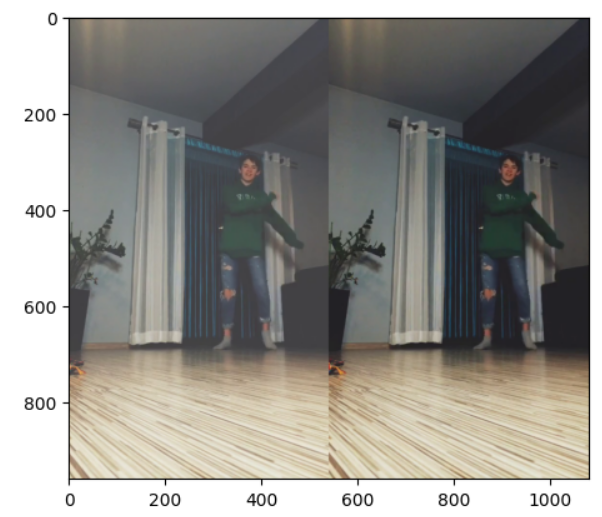
\includegraphics[width=.30\linewidth,valign=m]{constr_stretch} & 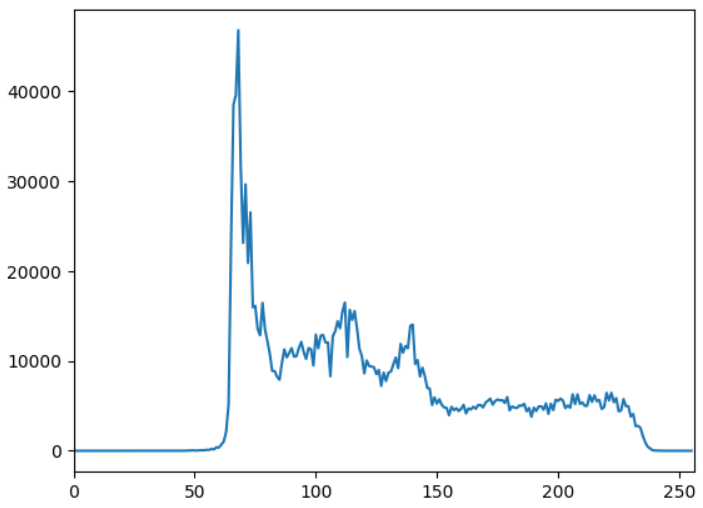
\includegraphics[width=.30\linewidth,valign=m]{hist_constr_stretch} & 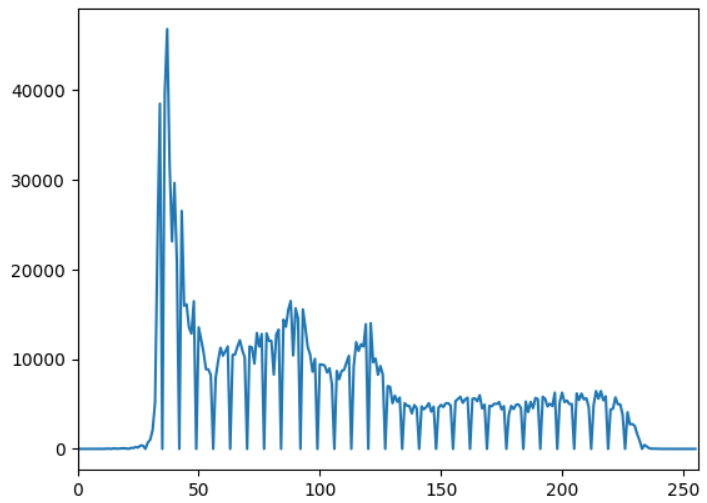
\includegraphics[width=.30\linewidth,valign=m]{hist_constr_stretch_1} 
\end{tabular}
\caption{\label{contr_stretch}Sample from Tik-Tok Segmentation Dataset pre-processed with contrast stretching.}
\end{table}

% bilateral filter image
\begin{table}[hbt!]
\centering
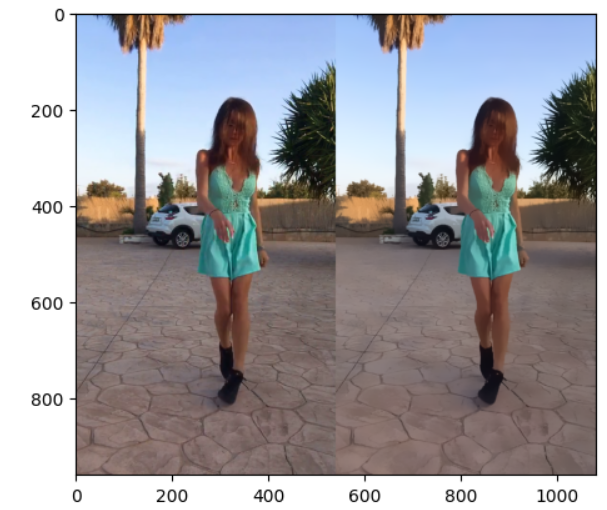
\includegraphics[width=.50\linewidth,valign=m]{bilateral_filtr}
\caption{\label{bil_fil}Sample from Tik-Tok Segmentation Dataset pre-processed with bilateral filter.}
\end{table}


% background removal images
\begin{table}[hbt!]
\centering
\begin{tabular}{cccc}
Ground-truth & 
\includegraphics[width=.15\linewidth,valign=m]{u-net-sample-1} & 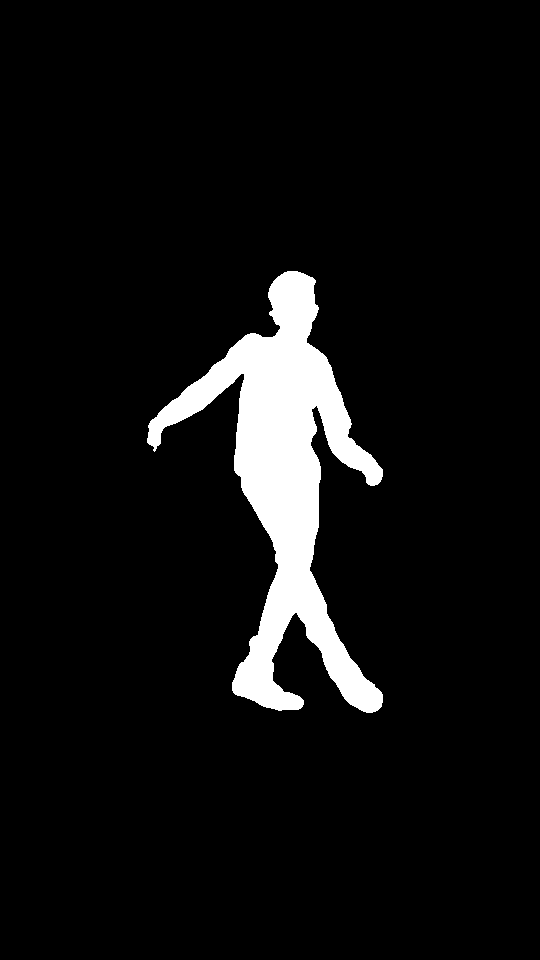
\includegraphics[width=.15\linewidth,valign=m]{u-net-sample-2} & 
\includegraphics[width=.15\linewidth,valign=m]{u-net-sample-3} \\ [0.5ex] 
 \hline\hline
Our results & 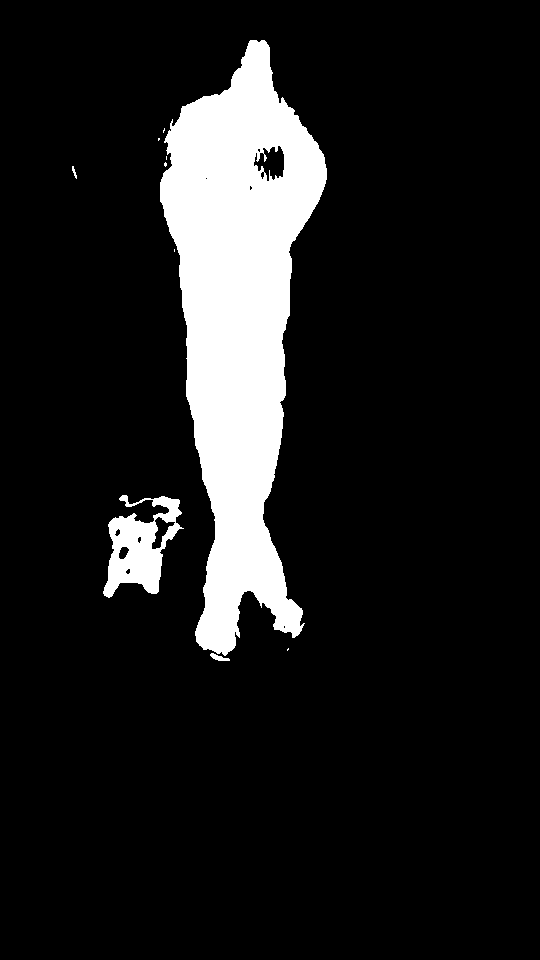
\includegraphics[width=.15\linewidth,valign=m]{u-net-sample-1-1} & 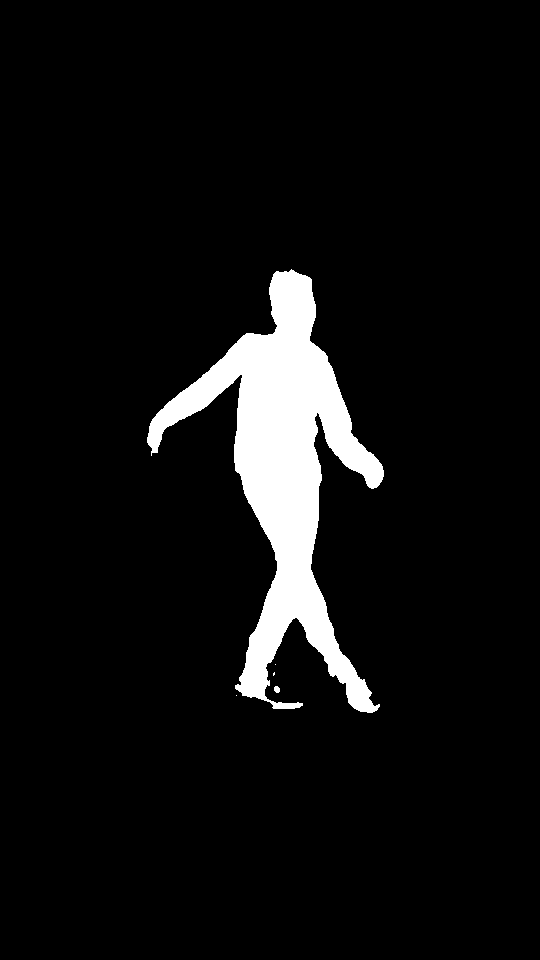
\includegraphics[width=.15\linewidth,valign=m]{u-net-sample-2-1}   & 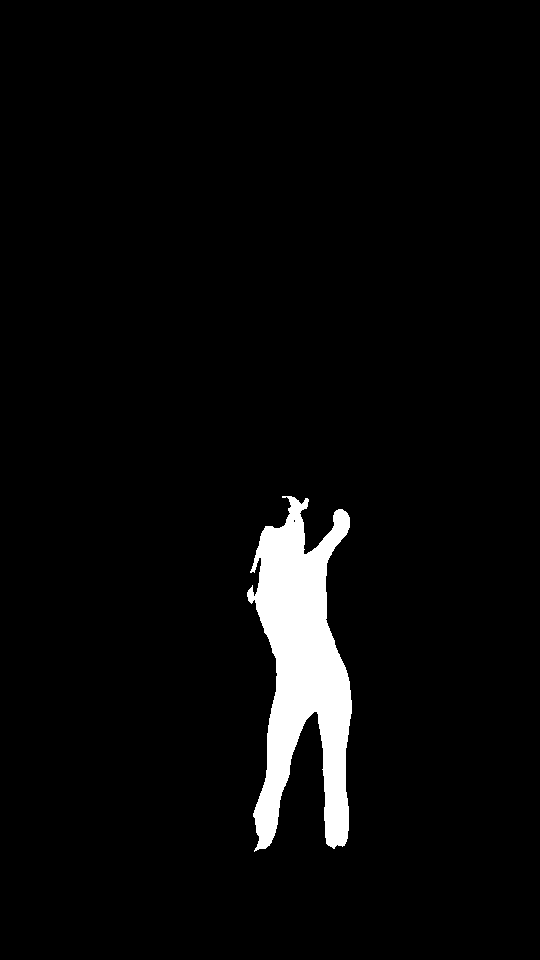
\includegraphics[width=.15\linewidth,valign=m]{u-net-sample-3-1} \\
\end{tabular}
\caption{\label{tiktok_dataset}Samples of segmentation maps from Tik-Tok Segmentation Dataset.}
\end{table}

\FloatBarrier


\begin{multicols}{2}

\subsection{Conclusion}
Cosa succederà nelle prossime puntate ?...?


\end{multicols}